\subsection{Edge crack in tension}

\paragraph{}
Consider a plate with an edge crack loaded in tension $\sigma=1N/m^2$ over the top and the bottom edges.
The geometry, loading and boundary conditions are shown in Fig.~\ref{iso_fig:edge_crack_geo_bc}.
In the figure, $L=2m$ and $H=1m$.
The reference mode \RN{1} SIF is given by:
    \begin{equation}
        K_1 = F\left(
            \frac{a}{H}
            \sigma \sqrt{\pi a}
        \label{iso_eq:edge_crack_k1}
        \right)
    \end{equation}
where $a$ is the crack length, $H$ is the plate width, and $F(a/H)$ is an empirical function given by (for $a/H \leq 0.6$)
    \begin{equation}
        F\left( \frac{a}{H} \right) =
            1.12 - 0.231 \left( \frac{a}{H} \right) +
            10.55\left( \frac{a}{H} \right)^2 -
            27.72\left( \frac{a}{H} \right)^3 +
            30.39\left( \frac{a}{H} \right)^4
    \end{equation}

    \begin{figure}
        \centering
        \scalebox{0.4}{
            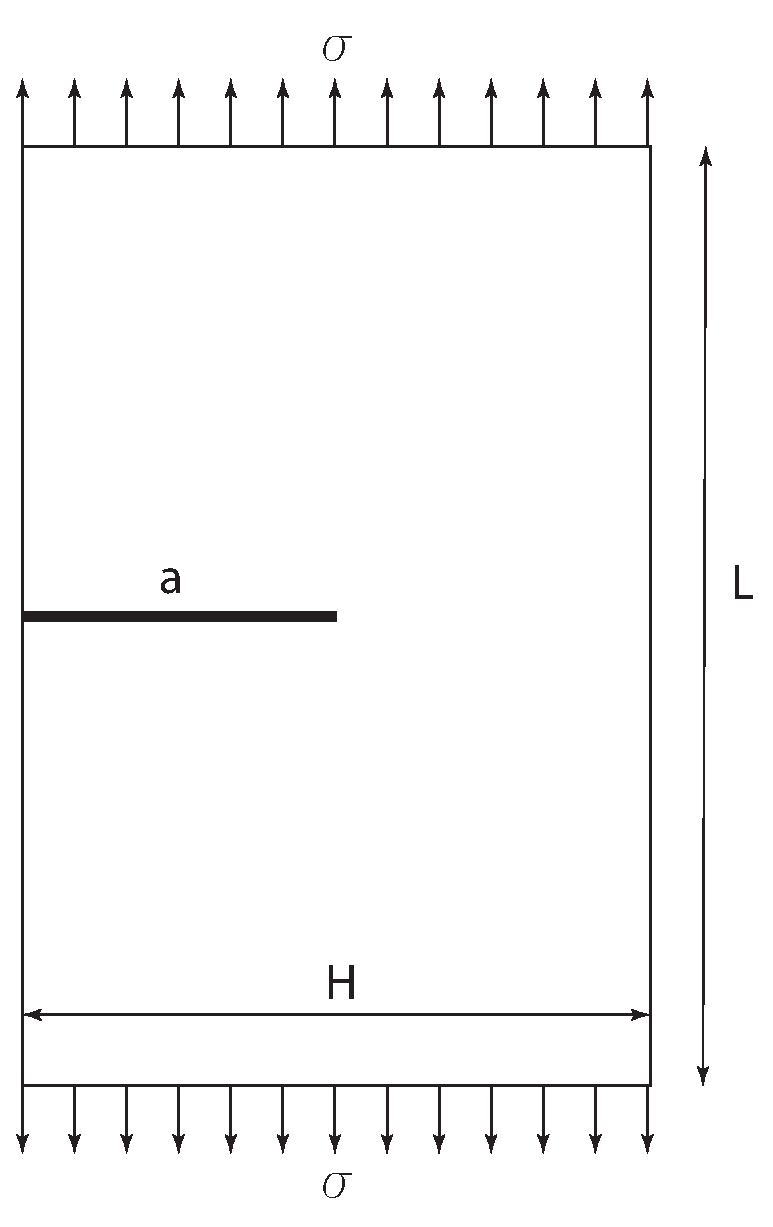
\includegraphics{isogeometric_sbfem/images/edge_crack_geo_bc.eps}
        }
        \caption{Plate with an edge crack under tension}
        \label{iso_fig:edge_crack_geo_bc}
    \end{figure}

\paragraph{}
The convergence of the mode \RN{1} SIF and the T-stress with the mesh size and the order of the NURBS basis function is illustrated in Tab.~\ref{iso_tab:edge_crack_res}.
It can be seen that decreasing the mesh size and increasing the order of the NURBS basis function, the numerically obtained SIF and the T-stress converge.
\begin{table}
    \caption{Convergence of the mode \RN{1} SIF and T-stress for an edge crack in tension}
    \label{iso_tab:edge_crack_res}
    \begin{tabularx}{\textwidth}{XXXXXXX}
        \toprule
            Total    &   \multicolumn{2}{c}{NURBS $p=2$} &\multicolumn{2}{c}{NURBS $p=4$} &\multicolumn{2}{c}{NURBS $p=6$}\\
            \cmidrule{2-7}
            DOF      &   $K_1$   &   T-stress            &$K_1$   &   T-stress            &$K_1$   &   T-stress           \\
            \cmidrule{1-1} \cmidrule{2-3} \cmidrule{4-5} \cmidrule{6-7}
            62       &   2.7011  &   -0.4137             &2.6647  &-0.4170                &        &                      \\
            98       &   2.7632  &   -0.4210             &2.8343  &-0.4216                &2.8335  &-0.4217               \\
            170      &   2.8028  &   -0.4216             &2.8252  &-0.4217                &2.8245  &-0.4217               \\
            329      &   2.8264  &   -0.4217             &2.8247  &-0.4217                &2.8246  &-0.4217               \\
            Eq.~\ref{iso_eq:edge_crack_k1} & 2.8264 & - & & & & \\
        \bottomrule
        \end{tabularx}
\end{table}

